\chapter{Conhecendo Suas Necessidades}

Antes de começar um projeto de mestrado ou doutorado, o aluno deve estar ciente de suas necessidades, limitações, restrições, capacidades e habilidades. Tudo isso deve ser levado em conta na sua preparação e mesmo na escolha se é o momento certo para realizar essa empreitada.

Em especial, quero chamar atenção às necessidades. Um trabalho de extrema repercussão é o estudo de Maslow  sobre a hierarquia de necessidades das pessoas\footnote{Esse trabalho também foi muito criticado, mas certamente podemos utilizá-lo para exemplificar o fato de que você tem que estar bem em vários sentidos para ter a calma necessária para fazer sua tese.}. Ele é facilmente compreendido a partir da “pirâmide de Maslow”, que apresento na Figura \ref{fig:maslow}.

\begin{figure}
	\centering
	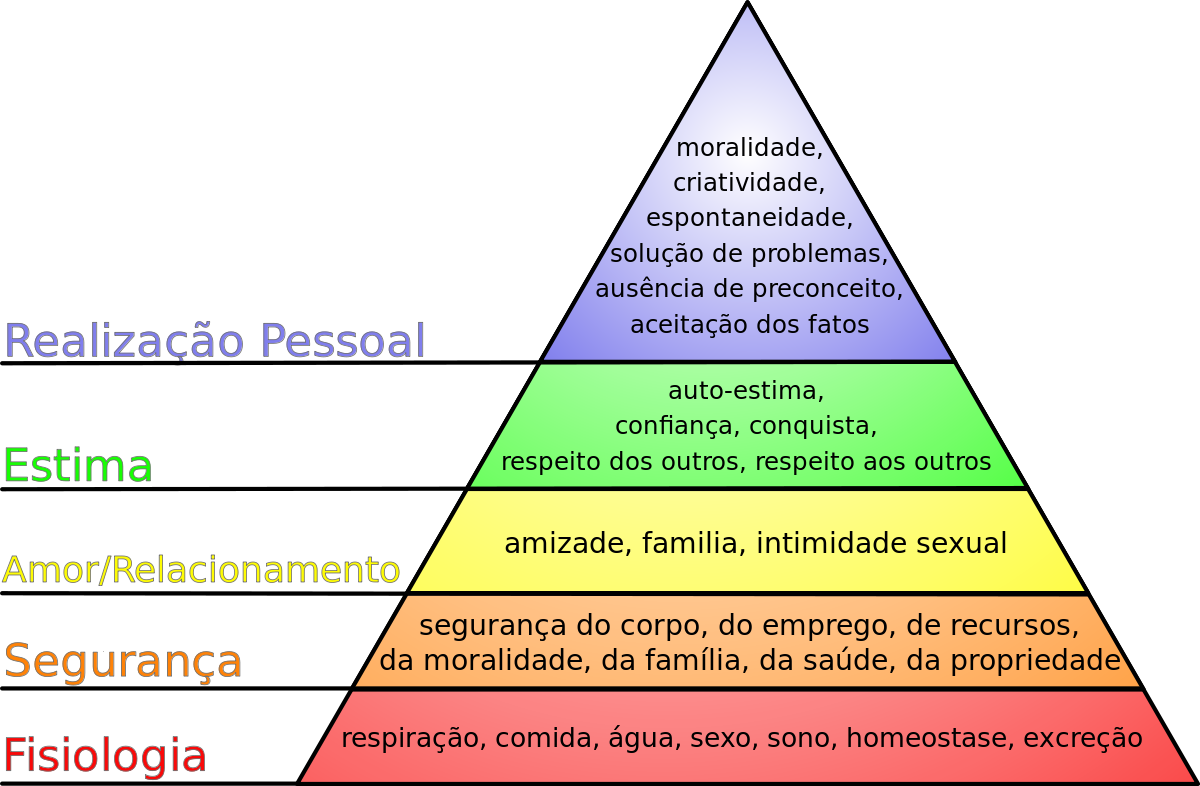
\includegraphics[width=0.7\linewidth]{Images/1200px-Hierarquia_das_necessidades_de_Maslow.svg}
	\caption{A pirâmide de Maslow.}
	\label{fig:maslow}
\end{figure}


Como se pode ver na Figura \ref{fig:maslow}, as necessidades são divididas em grupos e um grupo serve de base para todos os grupos superiores. Assim, as necessidades de realização pessoal (como fazer uma tese) são dependentes de todas as outras. 

Desse modo, podemos concluir que, para fazer uma pós-graduação, você deve garantir antes que tenha uma “boa base na pirâmide”. Isso significa garantir sua saúde, o modo de se manter, seus relacionamentos e sua autoestima.

Mesmo que você tenha começado sua dissertação ou tese em uma situação ideal, o longo prazo desse projeto, de 2 a 5 anos, implica em mudanças tanto no ambiente a sua volta quanto na sua própria vida. Alunos se casam, tem filhos, ficam doentes, se curam, precisam de mais dinheiro, se separam, trocam de emprego, tudo pode mudar nesse espaço de tempo.
Podemos citar como exemplo de acontecimento totalmente inesperado, e que afetou a todos em 2020/2021, a epidemia da Covid-19. Quantas vidas não foram mudadas? O impacto na vida dos mestrandos e graduandos foi muito variado e colocou um grande desafio para orientandos, orientadores e as instituições.

Voltando a pirâmide, ela indica que qualquer problema em uma camada inferior afeta diretamente a camada superior. Você deve estar consciente dessa estrutura e saber que problemas de qualquer tipo sempre afetarão seu rendimento na camada do topo, seja ocupando seu tempo, seja ocupando sua mente. Cabe ao aluno perceber e controlar o grau desse efeito, e quando necessário interagir com o orientador.

Por isso não hesite em procurar seu orientador e avisá-lo do que está acontecendo com você. Mesmo que ele não possa ajudá-lo no problema específico, ele compreenderá e tentará ajudar no que for possível. 
Exemplos típicos de coisas que acontecem na vida de um aluno: um novo emprego ou uma situação de desemprego, troca de chefes que afeta a liberação ou o interesse da empresa, doenças mais ou menos graves consigo ou com parentes, perda de acesso aos dados prometidos por alguém, gravidez, casamento, etc.

O orientador não é um sargento empurrando você em uma marcha forçada. Ao contrário, ele é o guia que evita que você se perca em uma exploração. Ele está ali para auxiliá-lo nos percalços do caminho, até mesmo para dizer que está na hora de parar e tentar em outra expedição. 
Uma relação aberta com o orientador é uma das mensagens que quero passar nesse texto. Ela vai facilitar sua vida e chegar ao seu objetivo.
